% !TEX encoding = UTF-8
% !TEX TS-program = pdflatex
% !TEX root = ../tesi.tex

%**************************************************************
\chapter{Contesto aziendale}
\label{cap:introduzione}
%**************************************************************

%**************************************************************
\section{Lab Network}

\begin{figure}[H]
	\begin{center}
	
\includegraphics[scale=0.4]{immagini/LOGO_LABNETWORK.png}
	\caption{Logo \lab{}}
	\end{center}
\end{figure}

\lab{} nasce nel 2016 con lo scopo di aiutare le imprese a creare e ad innovare prodotti e processi attraverso la competenza concreta dei laboratori, sfruttando le potenzialità dei moderni strumenti digitali.\\
L'azienda cerca di collaborare con più partners per poter ottenere una visione maggiore di prodotti e di conseguenza soddisfare i clienti.

\section{Organizzazione aziendale}
La start-up è attiva dal 24/01/2018 ed è composta da un amministratore unico e una dipendente.
L'organo amministrativo gestisce l'impresa e compie tutte le operazioni necessarie per il raggiungimento dell'oggetto sociale.
Le attività principali esercitate dallo staff sono:
\begin{itemize}
\item ideazione e gestione di sistemi informatici per la condivisione di conoscenze sulle nuove tecnologie ;
\item noleggio di macchine e attrezzature per ufficio;
\item commercio all'ingrosso di hardware e software;
\item noleggio di kit di formazione e materiale didattico innovativo (stampanti 3D, schede elettroniche, ecc..);
\item organizzazione e promozione di corsi di formazione per aziende e disoccupati;
\item partecipazione a fiere ed eventi di settore;
\item consulenza in ambito tecnologico e innovativo.
\end{itemize}
\subsection{Metodologia di lavoro e processi aziendali}
Lo schema che l'azienda ha sviluppato si divide in tre fasi:
\begin{itemize}
\item Creare l’interesse attraverso politiche di marketing discutendo di temi specifici ad alto impatto mediatico;
\item Raccogliere gruppi omogenei che condividono l'interesse ad una specifica tecnologia;
\item attraverso attività di consulenza e formazione si cerca da un lato di capire le esigenze produttive e dall’altro le potenzialità che una digitalizzazione (hardware o software) può contribuire alla crescita di una PMI.
\end{itemize}

\subsection{La metodologia agile}
\begin{figure}[H]
	\begin{center}
	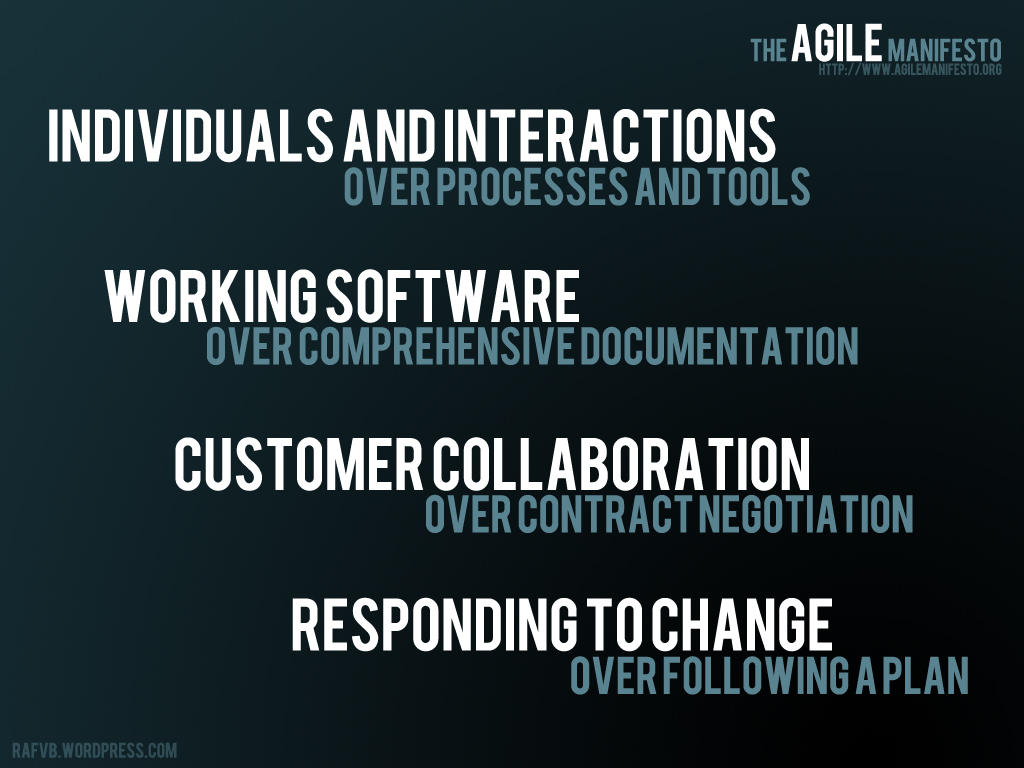
\includegraphics[scale=0.25]{immagini/agile_manifesto.jpg}
	\caption{I principi del manifesto agile}
	\end{center}
\end{figure}
\lab{} segue i principi della metodologia agile durante i processi di sviluppo di un nuovo progetto.
\begin{enumerate}
\item \textbf{Gli individui e le interazioni più che i processi e gli strumenti.}
\tab \lab{} infatti predilige una comunicazione.........
\item \textbf{Il software funzionante più che la documentazione esaustiva.}
\item \textbf{La collaborazione col cliente più che la negoziazione dei contratti.}
\item \textbf{Rispondere al cambiamento più che seguire un piano.}
\end{enumerate}




\subsection{Tecnologie}
Le principali tecnologie alle quali \lab{} si affida sono:
\begin{itemize}
\item Schede elettroniche (Arduino, Raspberry Pi, Intel UP Square, Asus TinkerBoard,…)
\item Stampanti 3D e software di progettazione CAD
\item Software di progettazione di ambienti VR (Unreal Engine, Unity…)
\item Applicazioni AR (Augmented Reality)
\item GitLab: piattaforma web open source che permette la gestione di repository Git e di funzioni trouble ticket
\item Protocollo Opc-Ua per l’automazione industriale 
\item Movidius Intel e strumenti per il Deep Learning e l’intelligenza artificiale
\item Android Studio e Xcode per lo sviluppo di applicazioni mobile
\item Blockchain e Criptovalute 
\item API per lo scambio dei dati
\end{itemize}

\newpage
\section{Prodotti e servizi}
\subsection{Prodotti}
\textbf{VITRUVIAN GAME – Wingsuit VR}
\\
Dalla collaborazione con Intel\textsuperscript{\textregistered} nasce il simulatore di volo con tuta alare ispirato al capolavoro di Leonardo.\\
Il progetto prevede l'utilizzo del visore HTC Vive affiancato ad uno scenario virtuale sviluppato su piattaforma \textit{Unity}. Per i movimenti sugli assi sono stati impiegati dei motori per automazione industriale.
\\
\\
\textbf{FabKey}
\\
La serratura smart connessa ad internet. Permette l'apertura di una porta controllando una lista di accessi presente in cloud. Funziona tramite tag \gls{NFC} o barcode. Il prodotto è rivolto principalmente ai \gls{FabLab}, ma si adatta facilmente a qualsiasi contesto in cui sia richiesto il controllo degli accessi.
\\
\\
\textbf{Smart Meter}
\\
Un metro 4.0 capace di misurare superfici complesse e inviare direttamente i dati al software gestionale, in aggiunta anche il monitoraggio in tempo reale di quando, dove e per quanto tempo è stato utilizzato dal singolo addetto.


\subsection{Servizi}
I servizi che \lab{} offre ai propri clienti sono:
\begin{itemize}
\item \textbf{Progettazione:} corsi di formazione su misura, \gls{counseling} e \gls{workshop} per imparare a sfruttare in modo professionale: 3D Printing, schede elettroniche, \gls{cz}, realtà virtuale e aumentata, sviluppo App, prototipazione, \gls{bigd}, \gls{iot} ecc.
\item \textbf{Noleggio:} Kit e attrezzature come stampanti 3D, schede elettroniche (\gls{arduino}, \gls{rpi}, Intel) visori VR, pc e notebook, videoproiettori; affitto aule didattiche per \gls{makers} e industria 4.0.
\item \textbf{Personale qualificato:} per i clienti sono a disposizione docenti, tecnici di laboratorio e consulenti specializzati nei principali ambiti di innovazione digitale.
\item \textbf{Assistenza:} pianificazione e costruzione su misura di progetti innovativi sviluppando idee imprenditoriali.
\end{itemize}

\section{Lab Network e innovazione}
\lab{} si è sviluppata nell’ambito della \textit{smart specialisation} attraverso logiche di coinvolgimento di una comunità di utenti misti che provengono prevalentemente dal mondo aziendale e accademico. 
\lab{} si propone come punto di riferimento per l’innovazione \textit{Open Source} nel territorio Veneto, tramite la rete interconnessa dei \gls{FabLab} esistenti, e promuovendosi come centro privilegiato di interscambio di conoscenza.\\
Comprendendo che il tessuto imprenditoriale Veneto è composto quasi totalmente di piccole e medie imprese dinamiche ed interconnesse, con un’industrializzazione diffusa ed una forte vocazione di tipo manifatturiero, \lab{} si è posta l’obiettivo di contribuire, attraverso strumenti e modalità di funzionamento specifici, a sviluppare ed attuare la strategia Regionale della ``Fabbrica Intelligente Del Futuro'', che mira ad indirizzare la trasformazione del settore manifatturiero verso nuovi prodotti, processi e tecnologie, attraverso lo sviluppo di attività di ricerca di alto livello.

\subsection{Smart Specialisation Strategy}
\begin{figure}[H]
	\begin{center}
	
\includegraphics[scale=0.4]{immagini/join-s3p.png}
	\caption{Logo della piattaforma della Smart Specialisation.}
	\small{\textbf{Fonte:} \url{http://s3platform.jrc.ec.europa.eu}}
	\end{center}
\end{figure}

La \textit{Smart Specialisation} è una strategia concepita nell'ambito della politica di coesione riformata dalla Commissione europea.\\
La specializzazione intelligente è un approccio fondato sull'individuazione di aree strategiche di intervento, basate sia sull'analisi dei punti di forza e del potenziale dell'economia sia su un processo di scoperta imprenditoriale con ampio coinvolgimento delle parti interessate.\\
Abbraccia un'ampia visione dell'innovazione, inclusi, ma certamente non limitati a, approcci basati sulla tecnologia e supportati da efficaci meccanismi di monitoraggio.\\
\\
\lab{} ha abbracciato questa strategia......
